% !TEX root = ./main.tex

\section{Introduction}\label{sec:project}

\subsection{Background}

\repoimages{} is a \langjulia image-processing toolbox that provides a collection of out-of-box functions\footnote{An overview of currently implemented image-processing functionalities is shown at \apicomparison.} to do image processing tasks just like \reposcikitimage{} and \matlabimageprocessing{} do.

However, despite the not yet benchmarked performance, this toolbox at present is still not friendly to both users and developers. Unlike other mature \langjulia{} packages such as \repojump and \repogpuarrays, \images{} requires potential users and developers to understand the very details of its mechanism and architecture, and this becomes even harder for them without comprehensive documentation on it. Under this circumstance, many image-processing researchers are still using \langpython and \langmatlab for their daily work.

Some apparent causes for its poor usability are:
{\normalsize
\begin{itemize}
    \item there are few demos or recipes in \images{} for new users to start with;
    \item APIs vary greatly across Images.jl submodules, and are unintuitive to the non-experts;
    \item there's no image-processing-specific style guide on naming and programming, except the \langjulia{} \href{https://docs.julialang.org/en/v1/manual/style-guide/}{style guide};
    \item there are many temporary helper functions and legacy codes everywhere;
    \item \images{} is an ecosystem but it lacks a comprehensive illustration of its packages;
    \item coverage of trait functions are not fully tested.
\end{itemize}
}
Fundamentally this is because the community is still in the progress of finding the most suitable programming style to process images using \langjulia. We can smell a bad code design from \cref{fig:imagetransformations_dep}, the dependency overview of \imagetransformations{}, where \imagecore{} doesn't play its core role well.

\begin{figure}[h]
  \centering
  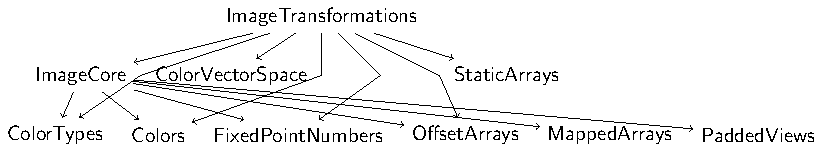
\includegraphics[width=0.8\textwidth]{figures/imagetransformations_dep.pdf}
  \caption{Dependency of \imagetransformations{}}\label{fig:imagetransformations_dep}
\end{figure}

Fortunately the problem is well-concerned in the community. Issues such as
{\small
\begin{itemize}
    \item \issue{\juliaimages}{\imagecore}{63} and \issue{\juliamath}{\fixedpointnumbers}{41} -- How to deal with overflow behavior of default \mintinline{julia}{N0f8} type?
    \item \issue{\juliaimages}{\images}{542} -- Roles of \sname{JuliaImages} documentation and \sname{Packages} documentation
    \item \issue{\juliaimages}{\images}{766} -- Use \mintinline{julia}{channelview} as possible as we can?
    \item \issue{\juliaimages}{\images}{767} -- Towards consistent style, part 1: a naming guide
    \item \issue{\juliaimages}{\images}{769} -- Goals of JuliaImages: Image types
    \item \issue{\juliaimages}{\images}{772} -- Revisiting the Images API
    \item \issue{\juliaimages}{\images}{790} -- Towards consistent style, part 2: a documentation guide
    \item \issue{\juliaimages}{\imagefeature}{46} -- Is \images{} just a convenient meta package?
    \item \issue{zygmuntszpak}{\imagebinarization}{23} -- What's the appropriate argument order?
    \item \issue{zygmuntszpak}{\imagebinarization}{24} -- Export limited number of symbols?
    \item \issue{zygmuntszpak}{\imagebinarization}{26} -- Filter specification: alternative to \mintinline{julia}{binarize}
\end{itemize}
}
discuss the coding styles and programming practice in the most generic way. \par

Packages such as \repohistogramthresholding and \repoimagebinarization are examples that validate the effectiveness and usefulness of style consensus reached in those issues. For instance, in \imagebinarization, one could binarize an image using any implemented methods\footnote{At the time of writing, there are 13 methods implemented.} with one unified API:
\mint{julia}{binarize(algo::BinarizationAlgorithm, img::AbstractArray)}
% end of subsection


\newpage
\subsection{Expectation}
With these existing work, it's in the right time to revisit the whole \images{} ecosystem and head towards a more easy-to-use \images{} package, and more ambitiously, towards \images{} \version{1.0}. This project aims to solve this problem by:
\begin{enumerate}
    \item providing more comprehensive and integrated documentation on both style guide and ecosystem illustration, and
    \item drafting RFCs (Request For Comments) and pruning code base of the ecosystem accordingly.
\end{enumerate}
Writing tutorials and demos of \images{} is not included in this project since it belongs to a totally different project. Trait functions will be tested and documented carefully to support high-level API design.

{\normalsize
This is a project on documentation and code refactoring to provide more consistent, robust and extensive APIs to both users and developers, and this is also a sub-project to \images{} \sname{v1.0} milestone. Potentially involved packages are:
\small
\begin{itemize}
    \item \textbf{user entrance:} \repoimages
    \item \textbf{core packages:} \repoimagecore, \repoimageaxes
    \item \textbf{application packages:} \repoimagemorphology, \repoimagetransformations, \repoimagedistance \repoimagemetadata and \repoimagefiltering
    \item \textbf{new packages\footnote{These packages are not yet imported by \images.}:} \repoimagebinarization, \repohistogramthresholding, \repoimageinpainting
\end{itemize}
\normalsize
Computer-vision packages (e.g., \repoimagetracking) and plotting packages (e.g., \repoimageview) are not under consideration of this project.\par}

While doing the documenting and code refactoring work, this project has many side effects:
{\normalsize
\begin{itemize}
    \item potential bug reports and patches to all related \langjulia repositories;
    \item introduction of new image processing packages (e.g., \sname{ImageEdge.jl}) to place legacy methods in \images;
    \item introduction of a new image denoising package, \repoimagenoise, as a concept-validation experimental field.\footnote{This is the author's research field.}
\end{itemize}
}
Note that these side effects are not counted as expectations of this project.\par

Before introducing the details of delivery schedule of this project, it's worth noting that workload and timeline of this project are hard to estimate due to the nature of this project:
\begin{itemize}
    \item this project can last for arbitrarily long time, and can contain an arbitrary number of issues and tasks; refactoring code base can last forever.
    \item lots of repositories are get involved in this project; time delay in receiving inputs from others is significant.
\end{itemize}
Hence the purpose of this project isn't to make the ecosystem perfect, instead, it is to evolve an ecosystem that is significantly better in API and naming style, so that future development towards \images{} \version{1.0} is possible.
